\begin{pastexam}[label={px:ntu-113-dsa-13}]{臺大資工所 113 學年度 第 13 題}
（問答；寫在試卷本上）

(30 points) A vertex cover of an undirected graph $G=(V,E)$ is a subset $V'\subseteq V$ such that if
$(u,v)\in E$, then either $u\in V'$ or $v\in V'$ (or both). The size of a vertex cover is defined as
the number of vertices in it. The vertex-cover problem is to find a vertex cover of minimum size in a
given undirected graph. It has been shown to be NP-hard, thus we cannot find a polynomial-time
algorithm for solving it exactly unless NP $=$ P. Fortunately, some polynomial-time approximation
algorithms have been proposed for solving the vertex-cover problem.

The following two approximation algorithms take as input an undirected graph and compute a vertex
cover for it. Initially, all edges in the graph are uncovered for both Algorithm VC-Arbitrary and
Algorithm VC-Max-Degree. Once a vertex $v$ is put into the cover, all edges incident on $v$ are
covered and removed.

Algorithm VC-Arbitrary picks an arbitrary uncovered edge $(u,v)$, puts both $u$ and $v$ into the
cover, throws out all edges incident on either $u$ or $v$, and repeats the process until there are no
uncovered edges left.

Algorithm VC-Max-Degree picks a vertex $v$ that covers the most number of uncovered edges, puts $v$
into the cover, throws out all edges incident on $v$, and repeats the process until there are no
uncovered edges left.
\begin{enumerate}[label=(\alph*)]
\item (10 points) Give an example for which Algorithm VC-Arbitrary yields a solution that is at least
double the size of a minimum-size vertex cover. Give another example for which Algorithm
VC-Max-Degree will definitely yield a solution with the size more than that of a minimum-size vertex
cover no matter how it breaks the tie. Each example should contain no more than ten vertices. You
have to justify your solution by showing the vertex cover found by the algorithm and its
corresponding minimum-size vertex cover.
\item (10 points) Prove or disprove that Algorithm VC-Arbitrary has a smaller ratio bound than
Algorithm VC-Max-Degree. The ratio bounds in your proof or disproof should be as tight as possible.
\item (10 points) In the weighted vertex-cover problem, you are given an undirected graph $G=(V,E)$
and a weight $w(v)$ for each vertex $v\in V$, and the objective is to find a vertex cover (covering all
edges in $E$) of minimum total weight. In other words, the goal is to find a vertex cover $C$ of $G$
such that $\sum_{v\in C}w(v)$ is minimized among all possible vertex covers of $G$. You are required
to formulate the weighted vertex cover problem as an integer linear program.
\end{enumerate}
\end{pastexam}

\begin{pastsoln}
VC-Arbitrary 就是資結書虛擬碼~29.1（只是邊的順序任意）；VC-Max-Degree 是資結書第~29.2~節的
「先拿度數最大的」。 (a)(b) 屬於近似演算法（本章），(c) 是整數線性規劃的建模。

\textbf{(a)} VC-Arbitrary 用完全二分圖 $K_{3,3}$：左邊 $a, b, c$，右邊 $x, y, z$，九條邊。 不論先挑哪條邊
$(u, v)$，$u$、$v$ 一左一右，拿掉它們的邊之後剩下 $K_{2,2}$；再挑一條剩下 $K_{1,1}$；再挑一條就沒有邊了。
所以不論怎麼挑，結果都是全部 $6$ 個點。 最小頂點覆蓋是 $3$：$\{a, b, c\}$ 蓋住所有邊；而
$(a, x), (b, y), (c, z)$ 三條邊沒有共用端點，至少要 $3$ 個點。 $6 = 2 \times 3$。

VC-Max-Degree 用資結書第~29.2~節的蜘蛛（$7$ 個點）：中心 $7$ 連到 $1, 2, 3$，再接 $(1,4)$、$(2,5)$、
$(3,6)$。
\begin{center}
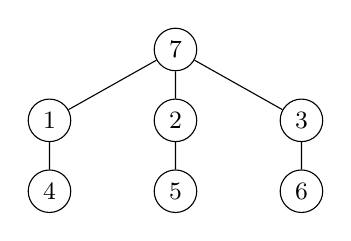
\begin{tikzpicture}[x=1cm,y=0.9cm,font=\small,n/.style={circle,draw,inner sep=0pt,minimum size=5.4mm}]
  \node[n] (c) at (0,0) {7};
  \node[n] (a) at (-1.6,-1) {1}; \node[n] (b) at (0,-1) {2}; \node[n] (d) at (1.6,-1) {3};
  \node[n] (a2) at (-1.6,-2) {4}; \node[n] (b2) at (0,-2) {5}; \node[n] (d2) at (1.6,-2) {6};
  \draw (c)--(a) (c)--(b) (c)--(d) (a)--(a2) (b)--(b2) (d)--(d2);
\end{tikzpicture}
\end{center}
第一步：$7$ 的度數是 $3$，$1, 2, 3$ 是 $2$，$4, 5, 6$ 是 $1$，最大的只有 $7$，沒有平手，一定先拿
$7$。 拿掉 $7$ 的三條邊之後，剩下 $(1,4)$、$(2,5)$、$(3,6)$ 三條互不相連的邊，每個點的度數都是 $1$；不論
平手怎麼取，每一步拿一條邊的一個端點、拿掉那條邊，共再拿 $3$ 個。 結果一定是 $4$ 個點，例如
$\{7, 1, 2, 3\}$。 最小頂點覆蓋是 $3$：$\{1, 2, 3\}$ 蓋住六條邊；$(1,4)$、$(2,5)$、$(3,6)$ 沒有共用端點，
至少要 $3$ 個。 $4 > 3$。

\textbf{(b)} 敘述成立：VC-Arbitrary 的近似比是 $2$，VC-Max-Degree 的近似比沒有常數上界，是
$\Theta(\log n)$。

VC-Arbitrary：資結書定理~29.1 證明了 $|C| \le 2|C^*|$（被挑的邊兩兩沒有共用端點，$C^*$ 至少要
$|M|$ 個點，而 $|C| = 2|M|$），證明不依賴挑邊的順序；(a) 的 $K_{3,3}$ 剛好是 $2$ 倍，所以 $2$ 是緊的。

VC-Max-Degree 的上界：它是不加權集合覆蓋的貪心（$X = E$，頂點 $v$ 對應它關聯的邊），由
資結書定理~29.5，$|C| \le H_\Delta |C^*| \le (\ln \Delta + 1)|C^*|$，$\Delta$ 是最大度數。

VC-Max-Degree 的下界：造一族二分圖 $G_k$，讓比值隨 $k$ 變大。 左邊 $k$ 個點 $a_1, \ldots, a_k$。 對每個
$i = 2, 3, \ldots, k$，把 $a_1, a_2, \ldots$ 從頭每 $i$ 個切成一組，切出 $\lfloor k/i \rfloor$ 組（尾巴不足
$i$ 個的不用），每一組加一個右邊的點，和組裡的 $i$ 個點相連；這些點叫第 $i$ 層，度數都是 $i$。 右邊一共
$|R| = \sum_{i=2}^{k} \lfloor k/i \rfloor$ 個點。 每個 $a_j$ 在每一層最多屬於一組，所以它的度數最多
$k - 1$。

\begin{itemize}
\item 貪心一定拿光右邊的點：用歸納法，設第 $k, k - 1, \ldots, i + 1$ 層已經拿完，第 $i$ 層拿了一部分。
這時第 $i$ 層還沒拿的點，鄰居都在左邊、都還沒被拿，度數仍是 $i$；第 $i$ 層以下的點度數 $< i$；每個
$a_j$ 剩下的邊只連到第 $2, \ldots, i$ 層，最多 $i - 1$ 條。 所以度數最大的只有第 $i$ 層的點，平手也只在
它們之間，貪心拿的一定是第 $i$ 層的點。 右邊的點全部拿完時，所有邊都被蓋住（每條邊都有一端在右邊），
貪心的答案是 $|R|$。
\item 最佳解 $\le k$：左邊 $k$ 個點蓋住所有邊。
\item 比值：$\lfloor k/i \rfloor \ge k/i - (i-1)/i > k/i - 1$，所以 $|R| > k(H_k - 1) - (k - 1) > k(H_k - 2)$，
比值 $|R|/k > H_k - 2$，隨 $k$ 變大而趨近無限大。 圖有 $n = k + |R| \le k H_k$ 個點，$\log n = \Theta(\log k)$，
所以比值是 $\Omega(\log n)$，和上界 $H_\Delta \le \ln n + 1$ 只差常數倍。
\end{itemize}

具體的例子是 $k = 16$：第 $2, 3, \ldots, 16$ 層各有 $8, 5, 4, 3, 2, 2, 2, 1, 1, 1, 1, 1, 1, 1, 1$ 個點，
$|R| = 34$。 貪心拿 $34$ 個點，左邊 $16$ 個點就夠，比值 $34/16 = 2.125 > 2$。

所以 VC-Arbitrary 的近似比 $2$ 比 VC-Max-Degree 的 $\Theta(\log n)$ 小，敘述成立。 注意這是最壞情況的比較；
在個別的圖上，VC-Max-Degree 常常比較好，例如星狀圖它只拿中心一個點，VC-Arbitrary 會拿兩個。

\textbf{(c)} 每個頂點 $v$ 設一個變數 $x_v$，$x_v = 1$ 表示 $v$ 放進覆蓋，$x_v = 0$ 表示不放：
\begin{align*}
\text{minimize}\quad & \sum_{v \in V} w(v)\, x_v \\
\text{subject to}\quad & x_u + x_v \ge 1 && \text{對每條邊 } (u, v) \in E, \\
& x_v \in \{0, 1\} && \text{對每個頂點 } v \in V.
\end{align*}
\textbf{為什麼對。} 頂點集合 $C$ 和 $0/1$ 向量 $x$ 一一對應：$x_v = 1 \iff v \in C$。 對一條邊 $(u, v)$，
$x_u + x_v \ge 1$ 恰好是「$u$、$v$ 至少一個在 $C$ 裡」，所以 $x$ 滿足所有限制式 $\iff$ $C$ 是頂點覆蓋；
目標函數 $\sum_v w(v) x_v$ 恰好是 $\sum_{v \in C} w(v)$。 於是整數線性規劃的最佳解 $x^*$ 對應的
$C^* = \{v \mid x^*_v = 1\}$ 就是最小權重的頂點覆蓋，兩者的最佳值相等。

補充：把 $x_v \in \{0, 1\}$ 放寬成 $0 \le x_v \le 1$ 就是線性規劃，可以在多項式時間解出；再把
$x_v \ge 1/2$ 的頂點放進覆蓋，每條邊的 $x_u + x_v \ge 1$ 保證至少一端 $\ge 1/2$，得到的是加權頂點覆蓋
的 $2$ 倍近似。 題目只要求寫出整數線性規劃，這段不是必要的。
\end{pastsoln}
